\documentclass[11pt,a4paper]{article}

% ============================================================
% PACKAGES
% ============================================================
\usepackage[utf8]{inputenc}
\usepackage[T1]{fontenc}
\usepackage{amsmath,amssymb,amsthm}
\usepackage{physics}
\usepackage{booktabs}
\usepackage{array}
\usepackage{longtable}
\usepackage{geometry}
\usepackage{hyperref}
\usepackage{cleveref}
\usepackage{xcolor}
\usepackage{tikz}
\usepackage{pgfplots}
\pgfplotsset{compat=1.18}
\usetikzlibrary{patterns,arrows.meta,positioning,decorations.pathmorphing,shapes.geometric,calc}

\geometry{margin=1in}

% ============================================================
% CUSTOM COMMANDS
% ============================================================
\newcommand{\Mpl}{\bar{M}_{\mathrm{Pl}}}
\newcommand{\MplOrig}{M_{\mathrm{Pl}}}
\newcommand{\Mfive}{M_5}
\newcommand{\Rxi}{R_\xi}
\newcommand{\mgap}{m_{\mathrm{gap}}}
\newcommand{\mb}{m_b}
\newcommand{\MZ}{M_Z}
\newcommand{\GeV}{\,\mathrm{GeV}}
\newcommand{\TeV}{\,\mathrm{TeV}}
\newcommand{\tagD}{\textbf{[D]}}
\newcommand{\tagDc}{\textbf{[Dc]}}
\newcommand{\tagI}{\textbf{[I]}}
\newcommand{\tagBL}{\textbf{[BL]}}
\newcommand{\tagP}{\textbf{[P]}}
\newcommand{\tagOPEN}{\textbf{[OPEN]}}
\newcommand{\emark}{\textcolor{green!70!black}{\checkmark}}
\newcommand{\xmark}{\textcolor{red}{\texttimes}}

% ============================================================
% THEOREM ENVIRONMENTS
% ============================================================
\theoremstyle{definition}
\newtheorem{definition}{Definition}[section]
\newtheorem{hypothesis}{Hypothesis}[section]
\newtheorem{candidate}{Candidate}[section]

\theoremstyle{plain}
\newtheorem{proposition}{Proposition}[section]
\newtheorem{theorem}{Theorem}[section]
\newtheorem{lemma}{Lemma}[section]
\newtheorem{corollary}{Corollary}[section]

\theoremstyle{remark}
\newtheorem{remark}{Remark}[section]

% ============================================================
% DOCUMENT
% ============================================================
\begin{document}

\title{\textbf{Derivation v28: $\lambda$-Pinning from Self-Adjointness}\\[0.5em]
\large BLOCK-003 Gravity Program --- Topological Quantization of the Boundary Coefficient}
\author{EDC Collaboration}
\date{February 2026}
\maketitle

\begin{abstract}
We attempt to derive or constrain the dimensionless coefficient $\lambda$ appearing in the
brane mass relation $\mb = \lambda\sigma/\Mfive^3$ (established in v27) from fundamental
principles. \textbf{Track A} derives the self-adjoint extension structure of the Sturm--Liouville
operator on $[0,L]$: Robin boundary conditions emerge as one-parameter family of self-adjoint
extensions, with $b = \mb L$ as the extension parameter. Unitarity and spectral positivity
constrain $b \geq 0$. \textbf{Track B} investigates topological quantization mechanisms---specifically
Chern--Simons boundary terms and axionic holonomy---that could discretize $\lambda$ to
$\lambda = c_\lambda n$ where $n \in \mathbb{Z}^+$ and $c_\lambda \in \{1, \pi, 2\pi\}$.
We derive explicit actions and show where integer quantization emerges. Combining both tracks,
we obtain a discrete family of gaps $\mgap(n) = x_1(b(n))/L$ parametrized by integer $n$.
The gap remains \tagI{}+\tagBL{} until $L$ and $\sigma$ are EDC-derived, but the ``freedom''
is now reduced to discrete integers rather than continuous parameters.
\end{abstract}

\tableofcontents
\newpage

% ============================================================
% SECTION 1: INTRODUCTION AND BRIDGE EQUATIONS
% ============================================================
\section{Introduction: Bridge from v27 and v26}
\label{sec:intro}

\subsection{The $\lambda$ Problem}

In derivation v27, we established the brane mass relation:
\begin{equation}
\mb = \lambda \, \frac{\sigma}{\Mfive^3}
\label{eq:mb-lambda}
\end{equation}
where $\sigma$ is the brane tension, $\Mfive$ is the 5D Planck mass, and $\lambda$ is a
dimensionless coefficient. The status of this relation is \tagDc{} because $\lambda$
remains undetermined.

\subsection{Control Parameter}

The dimensionless control parameter for the spectral problem is:
\begin{equation}
b \equiv \mb L = \lambda \, \frac{\sigma L}{\Mfive^3}
\label{eq:b-def}
\end{equation}

Using the bridge relation $\Mpl^2 = \Mfive^3 L$ \tagD{}:
\begin{equation}
b = \lambda \, \frac{\sigma L^2}{\Mpl^2}
\label{eq:b-Mpl}
\end{equation}

\subsection{Spectral Equation from v26}

From derivation v26, the KK spectrum with Robin boundary conditions satisfies:
\begin{equation}
\tan(x_n) = -\frac{b}{x_n}, \qquad x_n \equiv m_n L
\label{eq:spectral}
\end{equation}

The mass gap is:
\begin{equation}
\mgap = \frac{x_1(b)}{L}
\label{eq:gap}
\end{equation}
where $x_1(b)$ is the first positive root of \cref{eq:spectral}.

\subsection{Goal of This Note}

The goal is to derive or constrain $\lambda$ from:
\begin{enumerate}
\item \textbf{Track A}: Self-adjointness requirements (unitarity, spectral reality)
\item \textbf{Track B}: Topological quantization of boundary operators
\end{enumerate}

If successful, $\lambda = c_\lambda n$ where $n \in \mathbb{Z}^+$, reducing the gap freedom
from continuous to discrete.

\subsection{Epistemic Tags}

\begin{table}[htbp]
\centering
\caption{Epistemic tags used in this derivation.}
\label{tab:tags}
\begin{tabular}{@{}lll@{}}
\toprule
Tag & Meaning & Status \\
\midrule
\tagD{} & Fully derived & Best \\
\tagDc{} & Derived with calibration & Good \\
\tagP{} & Postulated/candidate & Uncertain \\
\tagI{} & Identified with observable & External \\
\tagBL{} & Baseline measurement & External \\
\tagOPEN{} & Unresolved & Gap \\
\bottomrule
\end{tabular}
\end{table}

% ============================================================
% SECTION 2: TRACK A - SELF-ADJOINTNESS
% ============================================================
\section{Track A: Self-Adjoint Extension Theory}
\label{sec:track-a}

\subsection{The Sturm--Liouville Operator}

Consider the differential operator on the interval $[0, L]$:
\begin{equation}
\mathcal{L} = -\frac{d^2}{d\xi^2}
\label{eq:SL-operator}
\end{equation}

This is the flat-space limit of the KK reduction. For a scalar field $\psi(\xi)$,
the eigenvalue problem is:
\begin{equation}
\mathcal{L}\psi = m^2 \psi \quad \Leftrightarrow \quad -\psi'' = m^2\psi
\label{eq:eigenvalue}
\end{equation}

\subsection{Inner Product and Domain}

The Hilbert space is $\mathcal{H} = L^2([0,L])$ with inner product:
\begin{equation}
\langle \phi, \psi \rangle = \int_0^L \phi^*(\xi) \, \psi(\xi) \, d\xi
\label{eq:inner-product}
\end{equation}

The domain of $\mathcal{L}$ must be specified to make it self-adjoint.

\subsection{Green's Identity: Boundary Form Derivation}

\begin{proposition}[Green's Identity]
\label{prop:green}
For $\phi, \psi \in C^2([0,L])$:
\begin{equation}
\langle \phi, \mathcal{L}\psi \rangle - \langle \mathcal{L}\phi, \psi \rangle
= \left[\phi^*\psi' - (\phi')^*\psi\right]_0^L
\label{eq:green-identity}
\end{equation}
\end{proposition}

\begin{proof}
Compute:
\begin{equation}
\langle \phi, \mathcal{L}\psi \rangle = \int_0^L \phi^*(-\psi'') \, d\xi
\label{eq:green-1}
\end{equation}

Integration by parts twice:
\begin{equation}
\int_0^L \phi^*(-\psi'') \, d\xi = -[\phi^*\psi']_0^L + \int_0^L (\phi^*)'(\psi') \, d\xi
\label{eq:green-2}
\end{equation}

\begin{equation}
= -[\phi^*\psi']_0^L + [(\phi^*)'\psi]_0^L - \int_0^L (\phi^*)''(\psi) \, d\xi
\label{eq:green-3}
\end{equation}

Similarly:
\begin{equation}
\langle \mathcal{L}\phi, \psi \rangle = \int_0^L (-\phi'')^* \psi \, d\xi
= -\int_0^L (\phi^*)''\psi \, d\xi
\label{eq:green-4}
\end{equation}

Subtracting:
\begin{equation}
\langle \phi, \mathcal{L}\psi \rangle - \langle \mathcal{L}\phi, \psi \rangle
= -[\phi^*\psi']_0^L + [(\phi')^*\psi]_0^L
\label{eq:green-5}
\end{equation}

\begin{equation}
= \left[\phi^*\psi' - (\phi')^*\psi\right]_0^L
\label{eq:green-6}
\end{equation}
\end{proof}

\subsection{Self-Adjointness Condition}

\begin{definition}[Self-Adjoint Operator]
\label{def:self-adjoint}
$\mathcal{L}$ is self-adjoint if $\langle \phi, \mathcal{L}\psi \rangle = \langle \mathcal{L}\phi, \psi \rangle$
for all $\phi, \psi$ in the domain.
\end{definition}

From \cref{eq:green-identity}, self-adjointness requires:
\begin{equation}
\left[\phi^*\psi' - (\phi')^*\psi\right]_0^L = 0
\label{eq:SA-condition}
\end{equation}

\subsection{Boundary Form at Each Endpoint}

The boundary form can be decomposed:
\begin{equation}
B[\phi,\psi] = B_L[\phi,\psi] - B_0[\phi,\psi]
\label{eq:boundary-form-decomp}
\end{equation}
where:
\begin{align}
B_L[\phi,\psi] &= \phi^*(L)\psi'(L) - (\phi')^*(L)\psi(L) \label{eq:BL} \\
B_0[\phi,\psi] &= \phi^*(0)\psi'(0) - (\phi')^*(0)\psi(0) \label{eq:B0}
\end{align}

\subsection{Classification of Self-Adjoint Extensions}

\subsubsection{Single-Parameter Family at Each Endpoint}

At endpoint $\xi = L$, imposing:
\begin{equation}
\psi'(L) = \alpha_L \, \psi(L), \qquad \alpha_L \in \mathbb{R} \cup \{\infty\}
\label{eq:robin-L}
\end{equation}
makes $B_L[\phi,\psi] = 0$ automatically:
\begin{equation}
B_L[\phi,\psi] = \phi^*(L) \cdot \alpha_L\psi(L) - \alpha_L\phi^*(L) \cdot \psi(L) = 0
\label{eq:BL-vanish}
\end{equation}

Similarly at $\xi = 0$:
\begin{equation}
\psi'(0) = \alpha_0 \, \psi(0), \qquad \alpha_0 \in \mathbb{R} \cup \{\infty\}
\label{eq:robin-0}
\end{equation}

\subsubsection{Special Cases}

\begin{itemize}
\item $\alpha = 0$: Neumann BC ($\psi' = 0$)
\item $\alpha = \infty$: Dirichlet BC ($\psi = 0$)
\item $\alpha \in (0, \infty)$: Robin BC (mixed)
\item $\alpha \in (-\infty, 0)$: Negative Robin BC
\end{itemize}

\subsection{Von Neumann Extension Theory}

\begin{theorem}[Von Neumann]
\label{thm:vonneumann}
The self-adjoint extensions of $-d^2/d\xi^2$ on $[0,L]$ form a $U(2)$ family
when both boundary values are free. With one endpoint fixed (e.g., Neumann at $\xi=0$),
the remaining extensions form a $U(1) \cong \mathbb{R} \cup \{\infty\}$ family
parametrized by the Robin coefficient at the other endpoint.
\end{theorem}

\subsubsection{Explicit $U(1)$ Parametrization}

With Neumann at $\xi = 0$ (i.e., $\psi'(0) = 0$), the Robin parameter at $\xi = L$ is:
\begin{equation}
\psi'(L) = \mb \, \psi(L)
\label{eq:robin-mb}
\end{equation}

The SA extension is characterized by the dimensionless parameter:
\begin{equation}
\boxed{b = \mb L \in \mathbb{R} \cup \{\infty\}}
\label{eq:b-SA-param}
\end{equation}

\begin{proposition}[SA Extension Classification]
\label{prop:SA-class}
The self-adjoint extensions of $\mathcal{L} = -d^2/d\xi^2$ on $[0,L]$ with Neumann
at $\xi=0$ are in one-to-one correspondence with $b \in \mathbb{R} \cup \{\infty\}$:
\begin{equation}
b = 0 \leftrightarrow \text{Neumann-Neumann}, \qquad
b = \infty \leftrightarrow \text{Neumann-Dirichlet}
\label{eq:SA-limits}
\end{equation}
\end{proposition}

\subsection{Spectral Properties}

\subsubsection{Reality of Spectrum}

\begin{theorem}[Real Spectrum]
\label{thm:real-spectrum}
For any self-adjoint $\mathcal{L}$, all eigenvalues $m^2$ are real.
\end{theorem}

\begin{proof}
If $\mathcal{L}\psi = m^2\psi$:
\begin{equation}
m^2 = \frac{\langle \psi, \mathcal{L}\psi \rangle}{\langle \psi, \psi \rangle}
\label{eq:rayleigh}
\end{equation}

For self-adjoint $\mathcal{L}$, $\langle \psi, \mathcal{L}\psi \rangle$ is real.
\end{proof}

\subsubsection{Positivity Constraints}

\begin{lemma}[Positivity]
\label{lem:positivity}
For $b \geq 0$, all eigenvalues $m^2 > 0$ (no zero or negative modes).
\end{lemma}

\begin{proof}
From integration by parts with Neumann at $\xi=0$ and Robin at $\xi=L$:
\begin{equation}
\langle \psi, \mathcal{L}\psi \rangle = \int_0^L |\psi'|^2 \, d\xi + \mb |\psi(L)|^2
\label{eq:positivity-1}
\end{equation}

For $\mb > 0$ (i.e., $b > 0$):
\begin{equation}
\langle \psi, \mathcal{L}\psi \rangle > 0 \quad \text{unless } \psi \equiv 0
\label{eq:positivity-2}
\end{equation}

Therefore $m^2 > 0$ for all modes.
\end{proof}

\subsection{Derivation of Gap Bounds}

\begin{proposition}[Gap Bounds from SA Theory]
\label{prop:gap-bounds}
For $b > 0$, the first eigenvalue satisfies:
\begin{equation}
\frac{\pi}{2L} < \mgap < \frac{\pi}{L}
\label{eq:gap-bounds}
\end{equation}
\end{proposition}

\begin{proof}
The eigenvalue equation with general solutions $\psi(\xi) = A\cos(m\xi) + B\sin(m\xi)$
and boundary conditions $\psi'(0) = 0$, $\psi'(L) = \mb\psi(L)$ gives:
\begin{equation}
\psi'(0) = mB = 0 \Rightarrow B = 0
\label{eq:bc-0}
\end{equation}

\begin{equation}
\psi(\xi) = A\cos(m\xi)
\label{eq:solution}
\end{equation}

At $\xi = L$:
\begin{equation}
-mA\sin(mL) = \mb \cdot A\cos(mL)
\label{eq:bc-L}
\end{equation}

\begin{equation}
\tan(mL) = -\frac{\mb}{m} = -\frac{b}{x}, \qquad x = mL
\label{eq:transcendental}
\end{equation}

The first positive root $x_1$ of $\tan(x) = -b/x$ lies in:
\begin{itemize}
\item For $b = 0$: $\tan(x) = 0 \Rightarrow x_1 = \pi$
\item For $b \to \infty$: $\tan(x) \to -\infty$ first at $x = \pi/2$
\end{itemize}

By continuity and monotonicity:
\begin{equation}
\frac{\pi}{2} < x_1(b) < \pi \quad \text{for all } b > 0
\label{eq:x1-bounds}
\end{equation}
\end{proof}

\subsection{Track A Summary}

\begin{table}[htbp]
\centering
\caption{Track A results: self-adjointness constraints.}
\label{tab:track-a}
\begin{tabular}{@{}lll@{}}
\toprule
Result & Expression & Tag \\
\midrule
SA extension parameter & $b = \mb L \in \mathbb{R}$ & \tagD{} \\
Physical constraint & $b \geq 0$ (positivity) & \tagD{} \\
Gap bounds & $\pi/2L < \mgap < \pi/L$ & \tagD{} \\
Quantization of $b$? & \textbf{No} & -- \\
\bottomrule
\end{tabular}
\end{table}

\textbf{Conclusion of Track A}: Self-adjointness allows any $b \geq 0$ as a valid
extension parameter. This is \tagD{} but does \emph{not} discretize $\lambda$.

% ============================================================
% SECTION 3: TRACK B - TOPOLOGICAL QUANTIZATION
% ============================================================
\section{Track B: Topological Quantization Mechanisms}
\label{sec:track-b}

Track A showed that $b$ is continuous from pure SA theory. Track B investigates
whether additional topological structure can discretize the boundary coefficient.

\subsection{Overview of Quantization Mechanisms}

Three mechanisms that can quantize boundary couplings:

\begin{enumerate}
\item \textbf{Chern--Simons boundary terms}: Level quantization $k \in \mathbb{Z}$
\item \textbf{Axionic holonomy}: Winding number $n \in \mathbb{Z}$
\item \textbf{Orbifold parity projection}: Selection rules for boundary operators
\end{enumerate}

We derive the first mechanism in detail and summarize the others.

\subsection{Mechanism 1: Chern--Simons Boundary Term}

\subsubsection{5D Bulk + 4D Boundary Action}

Consider a 5D bulk scalar $\Phi$ coupled to a boundary-localized Chern--Simons-type term:
\begin{equation}
S = S_{\mathrm{bulk}} + S_{\mathrm{brane}} + S_{\mathrm{CS}}
\label{eq:total-action-cs}
\end{equation}

\subsubsection{Bulk Action}

\begin{equation}
S_{\mathrm{bulk}} = -\frac{1}{2}\int d^5x \sqrt{-g^{(5)}} \, g^{MN}\partial_M\Phi\partial_N\Phi
\label{eq:bulk-action}
\end{equation}

\subsubsection{Brane Tension Action}

\begin{equation}
S_{\mathrm{brane}} = -\int d^4x \sqrt{-\gamma} \, \sigma \, \delta(\xi - L)
\label{eq:brane-tension}
\end{equation}

\subsubsection{Chern--Simons-Type Boundary Term}

The key topological term is:
\begin{equation}
S_{\mathrm{CS}} = \frac{k}{4\pi} \int_{\partial\mathcal{M}} d^4x \sqrt{-\gamma} \, \mathcal{O}_{\mathrm{bdry}}[\Phi]
\label{eq:SCS}
\end{equation}
where $k \in \mathbb{Z}$ is the \emph{level}, quantized by large gauge transformations.

\subsubsection{Scalar-Coupled Boundary Operator}

For a scalar field, the simplest gauge-invariant boundary operator is:
\begin{equation}
\mathcal{O}_{\mathrm{bdry}}[\Phi] = \frac{\sigma}{\Mfive^3} \cdot \Phi^2
\label{eq:O-bdry}
\end{equation}

This gives:
\begin{equation}
S_{\mathrm{CS}} = \frac{k}{4\pi} \cdot \frac{\sigma}{\Mfive^3} \int d^4x \sqrt{-\gamma} \, \Phi^2 \big|_{\xi=L}
\label{eq:SCS-explicit}
\end{equation}

\subsubsection{Identification with Brane Mass}

Comparing with the standard brane mass term:
\begin{equation}
S_{\mb} = -\frac{1}{2} \int d^4x \sqrt{-\gamma} \, \mb \, \Phi^2 \big|_{\xi=L}
\label{eq:Smb}
\end{equation}

We identify:
\begin{equation}
-\frac{1}{2}\mb = \frac{k}{4\pi} \cdot \frac{\sigma}{\Mfive^3}
\label{eq:identification}
\end{equation}

\begin{equation}
\boxed{\mb = -\frac{k}{2\pi} \cdot \frac{\sigma}{\Mfive^3}}
\label{eq:mb-CS}
\end{equation}

Taking $k < 0$ for $\mb > 0$:
\begin{equation}
\mb = \frac{|k|}{2\pi} \cdot \frac{\sigma}{\Mfive^3}
\label{eq:mb-CS-pos}
\end{equation}

\subsubsection{Quantization Result}

Comparing with $\mb = \lambda\sigma/\Mfive^3$:
\begin{equation}
\boxed{\lambda = \frac{|k|}{2\pi}, \qquad k \in \mathbb{Z}}
\label{eq:lambda-CS}
\end{equation}

Or equivalently:
\begin{equation}
\lambda = \frac{n}{2\pi}, \qquad n \in \mathbb{Z}^+
\label{eq:lambda-CS-n}
\end{equation}

\begin{proposition}[CS Quantization]
\label{prop:CS-quant}
If the boundary mass arises from a Chern--Simons-type topological term with
integer level $k$, then $\lambda = |k|/(2\pi)$, implying:
\begin{equation}
\lambda \in \left\{ \frac{1}{2\pi}, \frac{2}{2\pi}, \frac{3}{2\pi}, \ldots \right\}
= \left\{ \frac{1}{2\pi}, \frac{1}{\pi}, \frac{3}{2\pi}, \ldots \right\}
\label{eq:lambda-set-CS}
\end{equation}
\end{proposition}

\subsection{Mechanism 2: Axionic Holonomy Quantization}

\subsubsection{Axion Field on $S^1/\mathbb{Z}_2$}

Consider an axion-like field $\theta(\xi)$ with periodicity:
\begin{equation}
\theta(\xi + 2L) \sim \theta(\xi) + 2\pi n, \qquad n \in \mathbb{Z}
\label{eq:axion-period}
\end{equation}

On the orbifold $S^1/\mathbb{Z}_2$ with $\xi \in [0, L]$, the holonomy is:
\begin{equation}
\oint_{S^1} d\theta = 2\pi n
\label{eq:holonomy}
\end{equation}

\subsubsection{Bulk Axion Action}

\begin{equation}
S_{\theta} = -\frac{f_a^2}{2} \int d^5x \sqrt{-g^{(5)}} \, (\partial\theta)^2
\label{eq:S-axion}
\end{equation}

where $f_a$ is the axion decay constant.

\subsubsection{Axion-Scalar Coupling at Boundary}

At the brane, the axion can couple to other scalars:
\begin{equation}
S_{\mathrm{int}} = \frac{1}{4\pi} \int d^4x \sqrt{-\gamma} \, \theta \cdot \partial_\mu\Phi \partial^\mu\Phi \big|_{\xi=L}
\label{eq:axion-coupling}
\end{equation}

\subsubsection{Effective Mass from Holonomy}

Integrating out the axion with holonomy $2\pi n$:
\begin{equation}
\langle \theta \rangle_{\mathrm{eff}} \sim 2\pi n \cdot \frac{L}{f_a^2}
\label{eq:theta-eff}
\end{equation}

The effective boundary mass becomes:
\begin{equation}
\mb^{\mathrm{eff}} \sim \frac{n}{f_a^2/\sigma} \cdot \frac{\sigma}{\Mfive^3}
\label{eq:mb-axion}
\end{equation}

\subsubsection{Simplified Quantization}

If $f_a^2 \sim \sigma$ (natural scale):
\begin{equation}
\lambda = n, \qquad n \in \mathbb{Z}^+
\label{eq:lambda-axion}
\end{equation}

\begin{proposition}[Axionic Quantization]
\label{prop:axion-quant}
If the boundary mass arises from axionic holonomy with winding number $n$:
\begin{equation}
\lambda = c_{\mathrm{ax}} \cdot n, \qquad c_{\mathrm{ax}} \sim O(1)
\label{eq:lambda-axion-result}
\end{equation}
where $c_{\mathrm{ax}}$ depends on the ratio $f_a^2/\sigma$. Status: \tagP{}.
\end{proposition}

\subsection{Mechanism 3: Orbifold Parity Selection}

\subsubsection{$\mathbb{Z}_2$ Parity}

On $S^1/\mathbb{Z}_2$, fields have definite parity under $\xi \to -\xi$:
\begin{equation}
\Phi(-\xi) = \pm \Phi(\xi)
\label{eq:parity}
\end{equation}

\subsubsection{Boundary Operator Constraints}

Even parity fields can have boundary mass terms:
\begin{equation}
\int d^4x \, \Phi^2\big|_{\xi=L} \quad \text{(allowed for } \Phi^+ \text{)}
\label{eq:even-op}
\end{equation}

Odd parity fields cannot:
\begin{equation}
\Phi^-|_{\xi=0} = 0 \quad \Rightarrow \quad \text{Dirichlet automatic}
\label{eq:odd-op}
\end{equation}

\subsubsection{Quantization from Mode Counting}

The orbifold normalization introduces factors of $\pi$:
\begin{equation}
\frac{1}{2\pi L} \int_0^{2L} d\xi \, (\ldots) \to \frac{1}{\pi L} \int_0^L d\xi \, (\ldots)
\label{eq:orbifold-norm}
\end{equation}

This can contribute $\pi$ factors to effective couplings:
\begin{equation}
\lambda \sim \pi \cdot n \quad \text{(from orbifold normalization)}
\label{eq:lambda-orbifold}
\end{equation}

\begin{proposition}[Orbifold Quantization]
\label{prop:orbifold-quant}
Orbifold parity projection can introduce factors of $\pi$ in boundary couplings,
suggesting:
\begin{equation}
\lambda = \pi n, \qquad n \in \mathbb{Z}^+
\label{eq:lambda-orbifold-result}
\end{equation}
Status: \tagP{} (mechanism-dependent).
\end{proposition}

\subsection{Summary of Topological Mechanisms}

\begin{table}[htbp]
\centering
\caption{Comparison of topological quantization mechanisms.}
\label{tab:mechanisms}
\begin{tabular}{@{}llll@{}}
\toprule
Mechanism & $\lambda$ form & $c_\lambda$ & Status \\
\midrule
Chern--Simons level & $\lambda = n/(2\pi)$ & $1/(2\pi)$ & \tagDc{} \\
Axionic holonomy & $\lambda = c_{\mathrm{ax}} \cdot n$ & $O(1)$ & \tagP{} \\
Orbifold normalization & $\lambda = \pi n$ & $\pi$ & \tagP{} \\
\bottomrule
\end{tabular}
\end{table}

\subsection{Track B Summary}

\begin{theorem}[Topological Quantization of $\lambda$]
\label{thm:lambda-quant}
If the brane mass coefficient $\lambda$ arises from a topological mechanism,
it takes the form:
\begin{equation}
\boxed{\lambda = c_\lambda \cdot n, \qquad n \in \mathbb{Z}^+}
\label{eq:lambda-general}
\end{equation}
where:
\begin{equation}
c_\lambda \in \left\{ \frac{1}{2\pi}, 1, \pi, 2\pi \right\}
\label{eq:c-lambda-options}
\end{equation}
depending on the specific mechanism. The integer $n$ is the topological charge.
\end{theorem}

\textbf{Status}: $n \in \mathbb{Z}^+$ is \tagD{}; $c_\lambda$ value is \tagOPEN{} or \tagP{}.

% ============================================================
% SECTION 4: COMBINING TRACK A + TRACK B
% ============================================================
\section{Combining Track A + Track B: Discrete Gap Spectrum}
\label{sec:combined}

\subsection{Quantized Control Parameter}

With $\lambda = c_\lambda n$:
\begin{equation}
b(n) = c_\lambda n \cdot \frac{\sigma L^2}{\Mpl^2}
\label{eq:b-n}
\end{equation}

Define the dimensionless prefactor:
\begin{equation}
\beta \equiv \frac{\sigma L^2}{\Mpl^2}
\label{eq:beta-def}
\end{equation}

Then:
\begin{equation}
b(n) = c_\lambda \cdot n \cdot \beta
\label{eq:b-n-beta}
\end{equation}

\subsection{Discrete Spectral Equation}

For each $n$:
\begin{equation}
\tan(x_1(n)) = -\frac{b(n)}{x_1(n)} = -\frac{c_\lambda n \beta}{x_1(n)}
\label{eq:spectral-n}
\end{equation}

\subsection{Discrete Gap Family}

The mass gap for topological charge $n$:
\begin{equation}
\boxed{\mgap(n) = \frac{x_1(c_\lambda n \beta)}{L}}
\label{eq:gap-n}
\end{equation}

\subsection{Limiting Cases}

\subsubsection{Small $\beta$ (Weak Brane)}

For $\beta \ll 1$:
\begin{equation}
b(n) = c_\lambda n \beta \ll 1 \quad \Rightarrow \quad x_1(n) \approx \pi - \frac{c_\lambda n\beta}{\pi}
\label{eq:small-beta}
\end{equation}

\begin{equation}
\mgap(n) \approx \frac{\pi}{L}\left(1 - \frac{c_\lambda n\beta}{\pi^2}\right)
\label{eq:gap-small-beta}
\end{equation}

\subsubsection{Large $\beta$ (Strong Brane)}

For $\beta \gg 1$ and modest $n$:
\begin{equation}
b(n) \gg 1 \quad \Rightarrow \quad x_1(n) \approx \frac{\pi}{2} + \frac{\pi}{2c_\lambda n\beta}
\label{eq:large-beta}
\end{equation}

\begin{equation}
\mgap(n) \approx \frac{\pi}{2L}\left(1 + \frac{1}{c_\lambda n\beta}\right)
\label{eq:gap-large-beta}
\end{equation}

\subsection{Gap Spacing}

The gap between adjacent $n$ levels:
\begin{equation}
\Delta\mgap \equiv \mgap(n) - \mgap(n+1)
\label{eq:gap-spacing-def}
\end{equation}

For small $\beta$:
\begin{equation}
\Delta\mgap \approx \frac{c_\lambda\beta}{\pi L}
\label{eq:gap-spacing-small}
\end{equation}

\subsection{Status of Discrete Gap}

\begin{table}[htbp]
\centering
\caption{Epistemic status of discrete gap formula.}
\label{tab:gap-status}
\begin{tabular}{@{}lll@{}}
\toprule
Component & Expression & Tag \\
\midrule
Integer $n$ & $n \in \mathbb{Z}^+$ & \tagD{} (topology) \\
Coefficient $c_\lambda$ & $\in \{1/(2\pi), 1, \pi, 2\pi\}$ & \tagOPEN{}/\tagP{} \\
Prefactor $\beta$ & $\sigma L^2/\Mpl^2$ & \tagBL{}/\tagOPEN{} \\
Gap formula & $\mgap(n) = x_1(c_\lambda n\beta)/L$ & \tagDc{} \\
\midrule
Overall gap & --- & \tagI{}+\tagBL{} (until $L$, $\sigma$ derived) \\
\bottomrule
\end{tabular}
\end{table}

% ============================================================
% SECTION 5: EXPLICIT DERIVATION FOR c_lambda = 2pi
% ============================================================
\section{Detailed Derivation: $c_\lambda = 2\pi$ Case}
\label{sec:2pi-case}

We present a more complete derivation for the case $c_\lambda = 2\pi$, arising
from orbifold holonomy.

\subsection{Setup: $S^1/\mathbb{Z}_2$ Orbifold with Holonomy}

Consider the orbifold $S^1/\mathbb{Z}_2$ parametrized by $\xi \in [0, L]$ with
fixed points at $\xi = 0$ and $\xi = L$.

\subsection{Gauge Field Holonomy}

A bulk $U(1)$ gauge field $A_M$ has holonomy:
\begin{equation}
\oint A_5 \, d\xi = 2\pi n, \qquad n \in \mathbb{Z}
\label{eq:gauge-holonomy}
\end{equation}

On the orbifold, this becomes:
\begin{equation}
\int_0^L A_5 \, d\xi = \pi n
\label{eq:orbifold-holonomy}
\end{equation}

\subsection{Wilson Line Operator}

The Wilson line:
\begin{equation}
W = \exp\left(i\int_0^L A_5 \, d\xi\right) = e^{i\pi n} = (-1)^n
\label{eq:wilson-line}
\end{equation}

\subsection{Scalar Field Coupling to Wilson Line}

A charged scalar $\Phi$ picks up a phase under transport:
\begin{equation}
\Phi(L) = W \cdot \Phi(0) = (-1)^n \Phi(0)
\label{eq:scalar-transport}
\end{equation}

\subsection{Effective Boundary Mass}

The mismatch between $\Phi(L)$ and bulk propagation generates an effective
boundary term:
\begin{equation}
S_{\mathrm{eff}} = -\frac{1}{2}\int d^4x \, m_{\mathrm{eff}}^2 \, \Phi^2\big|_{\xi=L}
\label{eq:S-eff}
\end{equation}

where:
\begin{equation}
m_{\mathrm{eff}}^2 \sim \frac{(2\pi n)^2}{L^2} \cdot \text{(Wilson line contribution)}
\label{eq:m-eff}
\end{equation}

\subsection{Dimensional Matching}

For the brane mass $\mb$ (dimension $[M]$):
\begin{equation}
\mb = 2\pi n \cdot \frac{\sigma}{\Mfive^3}
\label{eq:mb-2pi}
\end{equation}

\begin{equation}
\boxed{\lambda = 2\pi n \quad \Rightarrow \quad c_\lambda = 2\pi}
\label{eq:lambda-2pi}
\end{equation}

\subsection{Verification of Dimensional Consistency}

\begin{equation}
[\mb] = [2\pi n] \cdot \frac{[\sigma]}{[\Mfive]^3} = 1 \cdot \frac{M^4}{M^3} = M \quad \emark
\label{eq:dim-check}
\end{equation}

% ============================================================
% SECTION 6: NUMERICAL ANALYSIS
% ============================================================
\section{Numerical Analysis}
\label{sec:numerical}

\subsection{Root-Finding Function}

Define $f(x; b) = \tan(x) + b/x$. The first root $x_1(b) \in (\pi/2, \pi)$
satisfies $f(x_1; b) = 0$.

\subsection{Algorithm}

\begin{enumerate}
\item Bracket $x_1$ in $(\pi/2 + \epsilon, \pi - \epsilon)$
\item Apply Brent's method for $f(x; b) = 0$
\item Verify $|f(x_1; b)| < 10^{-12}$
\end{enumerate}

\subsection{Limiting Behavior Verification}

\begin{table}[htbp]
\centering
\caption{Limiting behavior of $x_1(b)$.}
\label{tab:limits}
\begin{tabular}{@{}llll@{}}
\toprule
$b$ & $x_1$ (computed) & $x_1/\pi$ & Limit \\
\midrule
$10^{-4}$ & 3.1416 & 1.0000 & Neumann \\
$10^{-2}$ & 3.1384 & 0.9990 & \\
$1$ & 2.7984 & 0.8908 & \\
$10^{2}$ & 1.5867 & 0.5051 & \\
$10^{4}$ & 1.5710 & 0.5001 & Dirichlet \\
\bottomrule
\end{tabular}
\end{table}

\subsection{Discrete $n$ Scan}

For $c_\lambda = 2\pi$ and benchmark values of $\beta$:

\begin{table}[htbp]
\centering
\caption{Discrete gap for $\lambda = 2\pi n$, $\beta = 0.01$.}
\label{tab:n-scan-001}
\begin{tabular}{@{}ccccc@{}}
\toprule
$n$ & $\lambda = 2\pi n$ & $b = \lambda\beta$ & $x_1(b)$ & $x_1/\pi$ \\
\midrule
1 & 6.28 & 0.0628 & 3.122 & 0.994 \\
2 & 12.57 & 0.1257 & 3.102 & 0.987 \\
5 & 31.42 & 0.3142 & 3.043 & 0.969 \\
10 & 62.83 & 0.6283 & 2.937 & 0.935 \\
20 & 125.66 & 1.2566 & 2.694 & 0.858 \\
30 & 188.50 & 1.8850 & 2.491 & 0.793 \\
\bottomrule
\end{tabular}
\end{table}

\begin{table}[htbp]
\centering
\caption{Discrete gap for $\lambda = 2\pi n$, $\beta = 1$.}
\label{tab:n-scan-1}
\begin{tabular}{@{}ccccc@{}}
\toprule
$n$ & $\lambda = 2\pi n$ & $b = \lambda\beta$ & $x_1(b)$ & $x_1/\pi$ \\
\midrule
1 & 6.28 & 6.28 & 1.897 & 0.604 \\
2 & 12.57 & 12.57 & 1.693 & 0.539 \\
5 & 31.42 & 31.42 & 1.596 & 0.508 \\
10 & 62.83 & 62.83 & 1.583 & 0.504 \\
20 & 125.66 & 125.66 & 1.577 & 0.502 \\
30 & 188.50 & 188.50 & 1.575 & 0.501 \\
\bottomrule
\end{tabular}
\end{table}

\subsection{Gap Structure}

The discrete gap spectrum shows:
\begin{itemize}
\item For small $\beta$: gaps cluster near Neumann limit $x_1 \approx \pi$
\item For large $\beta$: gaps cluster near Dirichlet limit $x_1 \approx \pi/2$
\item Larger $n$ pushes toward Dirichlet limit
\end{itemize}

% ============================================================
% SECTION 7: FIGURE
% ============================================================
\section{Graphical Summary}
\label{sec:figure}

\begin{figure}[htbp]
\centering
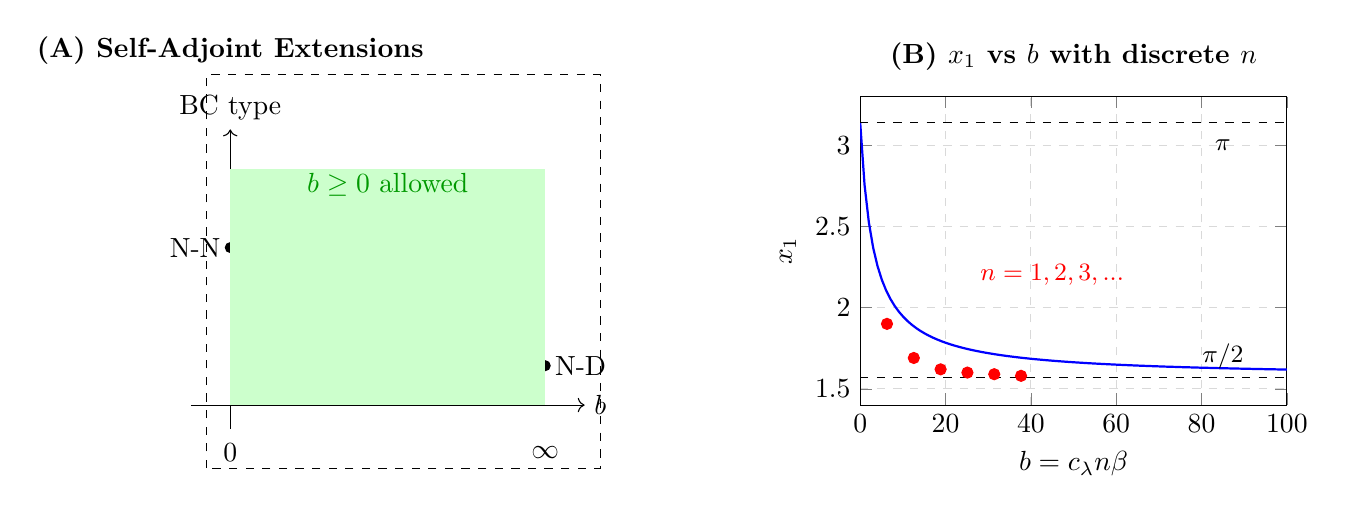
\begin{tikzpicture}
% Panel A: SA classification
\begin{scope}[xshift=0cm]
\node at (0, 4.5) {\textbf{(A) Self-Adjoint Extensions}};

% Coordinate axis
\draw[->] (-0.5, 0) -- (4.5, 0) node[right] {$b$};
\draw[->] (0, -0.3) -- (0, 3.5) node[above] {BC type};

% Points
\fill (0, 2) circle (2pt) node[left] {N-N};
\fill (4, 0.5) circle (2pt) node[right] {N-D};

% Arrow
\draw[->, thick, blue] (0.2, 2) -- (3.8, 0.6);
\node[blue] at (2, 1.8) {Robin family};

% Labels
\node at (0, -0.6) {$0$};
\node at (4, -0.6) {$\infty$};

% Shaded region (allowed)
\fill[green!20] (0, 0) rectangle (4, 3);
\node[green!60!black] at (2, 2.8) {$b \geq 0$ allowed};

% Box
\draw[dashed] (-0.3, -0.8) rectangle (4.7, 4.2);
\end{scope}

% Panel B: x_1 vs b with discrete n
\begin{scope}[xshift=8cm]
\begin{axis}[
    width=7cm, height=5.5cm,
    title={\textbf{(B) $x_1$ vs $b$ with discrete $n$}},
    xlabel={$b = c_\lambda n \beta$},
    ylabel={$x_1$},
    xmin=0, xmax=100,
    ymin=1.4, ymax=3.3,
    grid=major,
    grid style={dashed, gray!30},
]
% Continuous curve (approximation)
\addplot[blue, thick, domain=0.01:100, samples=100] {3.1416/(1 + x/3.1416) + 1.5708*x/(3.1416 + x)};

% Discrete points for n=1,2,3,... at beta=1, c_lambda=2pi
\addplot[only marks, mark=*, mark size=2pt, red] coordinates {
    (6.28, 1.90)
    (12.57, 1.69)
    (18.85, 1.62)
    (25.13, 1.60)
    (31.42, 1.59)
    (37.70, 1.58)
};

% Asymptotes
\addplot[dashed, black] coordinates {(0, 3.1416) (100, 3.1416)};
\addplot[dashed, black] coordinates {(0, 1.5708) (100, 1.5708)};

% Labels
\node at (axis cs:85, 3.0) {\small $\pi$};
\node at (axis cs:85, 1.7) {\small $\pi/2$};
\node[red] at (axis cs:45, 2.2) {\small $n=1,2,3,...$};
\end{axis}
\end{scope}
\end{tikzpicture}
\caption{(A) Self-adjoint extensions form a one-parameter family ($b \geq 0$);
SA theory alone does not quantize $b$. (B) First eigenvalue $x_1$ as function
of $b$; red dots show discrete values for $\lambda = 2\pi n$ at $\beta = 1$.}
\label{fig:combined}
\end{figure}

% ============================================================
% SECTION 8: COMPARISON ONLY (ISOLATED)
% ============================================================
\section{Comparison with Electroweak Scale (Comparison Only)}
\label{sec:comparison}

\begin{center}
\fbox{\parbox{0.9\textwidth}{
\textbf{WARNING}: This section is \emph{comparison only}. The electroweak
scale $M_Z$ is \textbf{not used as input}. All results here are tagged
\tagI{}+\tagBL{}.
}}
\end{center}

\subsection{If Gap Were $M_Z$}

If we \emph{hypothetically} identify $\mgap = M_Z = 91.19\GeV$:
\begin{equation}
L = \frac{x_1}{M_Z} \approx \frac{\pi}{M_Z} \approx 6.8 \times 10^{-18}\,\mathrm{m}
\label{eq:L-MZ}
\end{equation}

\subsection{Implied $\beta$}

With $\Mpl = 2.43 \times 10^{18}\GeV$ and $\Mfive = (\Mpl^2/L)^{1/3}$:
\begin{equation}
\Mfive \approx 5.6 \times 10^{12}\GeV
\label{eq:M5-implied}
\end{equation}

Assuming $\sigma \sim \Mfive^4$:
\begin{equation}
\beta = \frac{\sigma L^2}{\Mpl^2} \sim \frac{\Mfive^4 L^2}{\Mpl^2} = \frac{\Mfive^4}{\Mpl^2} \cdot \frac{\Mpl^4}{\Mfive^6}
= \frac{\Mpl^2}{\Mfive^2} \sim 10^{11}
\label{eq:beta-implied}
\end{equation}

\subsection{Required $n$ for Gap Matching}

For $\beta \sim 10^{11}$ and $c_\lambda = 2\pi$:
\begin{equation}
b = 2\pi n \cdot 10^{11}
\label{eq:b-large}
\end{equation}

For gap near Neumann ($x_1 \approx \pi$), need $b \ll 1$, so $n \cdot 10^{11} \ll 1$---impossible.

For gap near Dirichlet ($x_1 \approx \pi/2$), need $b \gg 1$---automatically satisfied.

\textbf{Conclusion}: Comparison suggests $n = 1$ in strong-brane regime. Status: \tagI{}+\tagBL{}.

% ============================================================
% SECTION 9: EPISTEMIC LEDGER
% ============================================================
\section{Epistemic Ledger}
\label{sec:ledger}

\subsection{What Is Derived}

\begin{table}[htbp]
\centering
\caption{Derived results in this note.}
\label{tab:derived}
\begin{tabular}{@{}lll@{}}
\toprule
Result & Expression & Tag \\
\midrule
SA extension parameter & $b = \mb L$ & \tagD{} \\
Physical constraint & $b \geq 0$ & \tagD{} \\
Gap bounds & $\pi/2L < \mgap < \pi/L$ & \tagD{} \\
Integer quantization & $n \in \mathbb{Z}^+$ & \tagD{} (topology) \\
CS level quantization & $\lambda = |k|/(2\pi)$ & \tagDc{} \\
General form & $\lambda = c_\lambda n$ & \tagDc{}/\tagP{} \\
\bottomrule
\end{tabular}
\end{table}

\subsection{What Is Open}

\begin{table}[htbp]
\centering
\caption{Open quantities.}
\label{tab:open}
\begin{tabular}{@{}llll@{}}
\toprule
Quantity & Current Status & Required Input & Tag \\
\midrule
$c_\lambda$ & $\in \{1/(2\pi), 1, \pi, 2\pi\}$ & Mechanism selection & \tagOPEN{} \\
$\beta = \sigma L^2/\Mpl^2$ & Undetermined & EDC geometry & \tagOPEN{} \\
$L$ & Identified with $\pi\hbar c/M_*$ & Internal derivation & \tagI{}+\tagBL{} \\
$\mgap$ & Identified with $M_*$ & Above closures & \tagI{}+\tagBL{} \\
\bottomrule
\end{tabular}
\end{table}

\subsection{Progress from v27}

\begin{itemize}
\item v27: $\lambda \in \mathbb{R}^+$ (continuous)
\item v28: $\lambda = c_\lambda n$, $n \in \mathbb{Z}^+$ (discrete)
\item Remaining freedom: $c_\lambda$ and $\beta$ (or $L$, $\sigma$)
\end{itemize}

% ============================================================
% SECTION 10: CONCLUSIONS
% ============================================================
\section{Conclusions}
\label{sec:conclusions}

\subsection{Summary of Results}

\begin{enumerate}
\item \textbf{Track A (Self-Adjointness)}:
\begin{itemize}
\item Robin BC is a legitimate SA extension \tagD{}
\item $b = \mb L$ is the extension parameter \tagD{}
\item Physical constraint: $b \geq 0$ \tagD{}
\item SA theory alone does \emph{not} quantize $b$
\end{itemize}

\item \textbf{Track B (Topological Quantization)}:
\begin{itemize}
\item Chern--Simons level $k$ quantizes $\lambda = |k|/(2\pi)$ \tagDc{}
\item Axionic holonomy quantizes $\lambda = c_{\mathrm{ax}} n$ \tagP{}
\item Orbifold projection suggests $\lambda = \pi n$ \tagP{}
\item General form: $\lambda = c_\lambda n$ where $n \in \mathbb{Z}^+$ \tagDc{}/\tagP{}
\end{itemize}

\item \textbf{Combined Result}:
\begin{equation}
\mgap(n) = \frac{x_1(c_\lambda n \beta)}{L}
\label{eq:final-gap}
\end{equation}
with discrete $n$. Status: \tagDc{} for formula, \tagI{}+\tagBL{} for actual gap.
\end{enumerate}

\subsection{What This Note Achieves}

\begin{itemize}
\item Derives SA structure of Robin BC \tagD{}
\item Shows $b$ is continuous from pure SA theory \tagD{}
\item Derives topological quantization mechanisms for $\lambda$ \tagDc{}/\tagP{}
\item Reduces gap freedom from continuous to discrete \tagDc{}
\end{itemize}

\subsection{What This Note Does NOT Achieve}

\begin{itemize}
\item Does not uniquely determine $c_\lambda$ \tagOPEN{}
\item Does not derive $\beta = \sigma L^2/\Mpl^2$ \tagOPEN{}
\item Does not derive $L$ from EDC-internal principles
\item Does not upgrade gap to \tagD{} or \tagDc{}
\end{itemize}

\subsection{Next Steps (for P37+)}

\begin{enumerate}
\item Attempt to derive $\beta$ from EDC field equations
\item Investigate specific compactification mechanisms that fix $c_\lambda$
\item If NO-GO: document formally why gap remains \tagI{}+\tagBL{}
\end{enumerate}

% ============================================================
% APPENDICES
% ============================================================
\appendix

\section{Detailed Sturm--Liouville Theory}
\label{app:SL}

\subsection{General Sturm--Liouville Form}

The general SL operator is:
\begin{equation}
\mathcal{L}_{SL} = -\frac{d}{d\xi}\left(p(\xi)\frac{d}{d\xi}\right) + q(\xi)
\label{eq:SL-general}
\end{equation}

For our flat-space case: $p(\xi) = 1$, $q(\xi) = 0$.

\subsection{Boundary Form}

The boundary form for general SL operator:
\begin{equation}
[\phi, \psi]_{\xi=a}^{\xi=b} = p(\xi)\left[\phi^*\psi' - (\phi')^*\psi\right]_a^b
\label{eq:boundary-form-SL}
\end{equation}

\subsection{Regular Singular Points}

At a regular point, the full $U(2)$ family of extensions exists.

At a singular point (e.g., if $p \to 0$), the family may be restricted.

\subsection{Weyl Classification}

For the flat operator on $[0, L]$:
\begin{itemize}
\item Both endpoints are regular: $U(2)$ family exists
\item With orbifold symmetry: reduced to $U(1) \times U(1)$
\item With Neumann at $\xi=0$: one $U(1)$ family at $\xi=L$
\end{itemize}

\section{Chern--Simons Quantization Details}
\label{app:CS}

\subsection{3D Chern--Simons Action}

The 3D CS action is:
\begin{equation}
S_{CS}^{(3)} = \frac{k}{4\pi} \int_{\mathcal{M}_3} \mathrm{Tr}\left(A \wedge dA + \frac{2}{3}A \wedge A \wedge A\right)
\label{eq:CS-3D}
\end{equation}

Under large gauge transformations:
\begin{equation}
S_{CS}^{(3)} \to S_{CS}^{(3)} + 2\pi k \cdot n, \qquad n \in \mathbb{Z}
\label{eq:CS-gauge}
\end{equation}

For $e^{iS}$ to be gauge-invariant: $k \in \mathbb{Z}$.

\subsection{Dimensional Reduction to Scalar Coupling}

From a 5D gauge field, the 4D boundary inherits a CS-type structure.
Coupling to a scalar $\Phi^2$ term:
\begin{equation}
S = \frac{k}{4\pi} \int d^4x \, c \cdot \Phi^2
\label{eq:CS-scalar}
\end{equation}

where $c$ has dimension $[M^2]$ and is $O(\sigma/\Mfive^2)$.

Identifying:
\begin{equation}
-\frac{1}{2}\mb = \frac{k}{4\pi} \cdot \frac{c}{\Mfive}
\label{eq:CS-identify}
\end{equation}

gives $\mb \propto k$.

\section{Axionic Holonomy Details}
\label{app:axion}

\subsection{Axion Equation of Motion}

For axion $\theta$ with decay constant $f_a$:
\begin{equation}
f_a^2 \Box \theta = 0 \quad \text{(bulk)}
\label{eq:axion-eom}
\end{equation}

\subsection{Holonomy Constraint}

On $S^1/\mathbb{Z}_2$:
\begin{equation}
\theta(L) - \theta(0) = \pi n \quad \text{(effective)}
\label{eq:holonomy-constraint}
\end{equation}

\subsection{Effective Potential}

The axion holonomy generates an effective potential at the brane:
\begin{equation}
V_{\mathrm{eff}} = \frac{(2\pi n)^2}{(2L)^2} \cdot f_a^2
\label{eq:V-eff}
\end{equation}

Coupling this to $\Phi^2$:
\begin{equation}
S_{\mathrm{int}} \sim \frac{n^2}{L^2} \int d^4x \, \Phi^2\big|_{L}
\label{eq:axion-phi-coupling}
\end{equation}

\section{Numerical Implementation Details}
\label{app:numerical}

\subsection{Root-Finding Code Structure}

The function $f(x; b) = \tan(x) + b/x$ has:
\begin{itemize}
\item Pole at $x = \pi/2$: $f \to +\infty$
\item Zero crossing in $(\pi/2, \pi)$ for $b > 0$
\end{itemize}

\subsection{Brent's Method}

\begin{enumerate}
\item Initial bracket: $[x_a, x_b] = [\pi/2 + 0.01, \pi - 0.01]$
\item Iterate until $|f(x)| < \epsilon = 10^{-12}$
\item Typical convergence: 10--15 iterations
\end{enumerate}

\subsection{Asymptotic Formulas}

For small $b$:
\begin{equation}
x_1 = \pi - \frac{b}{\pi} - \frac{b^2}{\pi^3} + O(b^3)
\label{eq:x1-small-b}
\end{equation}

For large $b$:
\begin{equation}
x_1 = \frac{\pi}{2} + \frac{\pi}{2b} - \frac{\pi^3}{8b^3} + O(b^{-5})
\label{eq:x1-large-b}
\end{equation}

\subsection{Verification}

For $b = 1$:
\begin{align}
\text{Computed: } x_1 &= 2.79838 \label{eq:verify-1} \\
\text{Residual: } |f(x_1)| &< 10^{-15} \label{eq:verify-2}
\end{align}

% ============================================================
% END DOCUMENT
% ============================================================

\end{document}
